\textbf{COLUNI 2023 -- Questão 27}\par\medskip Todos os organismos são formados por uma ou mais células e todas elas provém de outras células. Nos organismos pluricelulares, como o ser humano, as células possuem funções especializadas, diferentemente do que ocorre em uma ameba, organismo em que uma única célula realiza todas as funções necessárias à vida. Células animais apresentam estruturas, mostradas na figura abaixo, com funções bem definidas.

% COLUNI-AUTO-FIGURES-BEGIN
\begin{figure}[htbp]
\centering
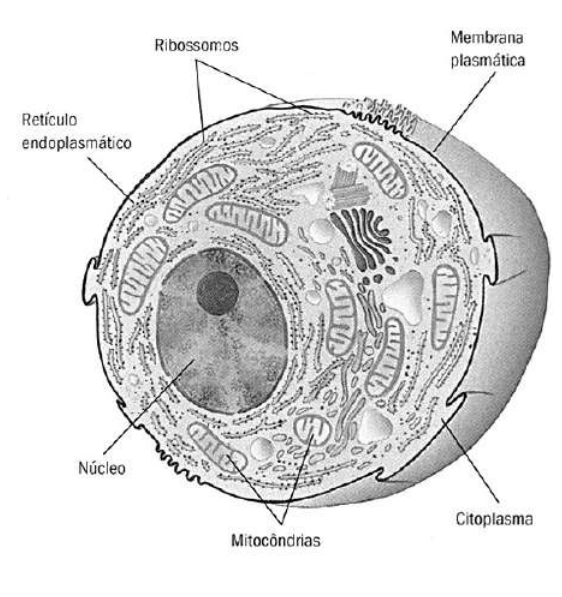
\includegraphics[width=0.95\linewidth]{static/simulados/coluni/figuras/2023/questao-27/figura-1.png}
\end{figure}
% COLUNI-AUTO-FIGURES-END
\begin{center}
Figura em corte de uma célula animal genérica, com base em observações feitas ao microscópio eletrônico.\\
Fonte: SILVA JÚNIOR, C.; SASSON, S.; SANCHES, P. S. B. \textbf{Ciência Entendendo a Natureza}, 8º ano. São Paulo: Editora Saraiva, 2013. p. 32.
\end{center}

Sobre as estruturas representadas da célula animal e suas funções, é INCORRETO afirmar:
\begin{enumerate}
\item A membrana plasmática, fina e de composição lipoproteica, reveste toda célula animal e regula as trocas
        de substâncias entre a célula e o meio externo.
\item Os ribossomos são pequenas estruturas que participam do processo de síntese de proteínas e podem
        estar livres no citoplasma ou associados às membranas do retículo endoplasmático.
\item As mitocôndrias utilizam determinadas substâncias como fontes de energia e, durante o processo de
        respiração celular, disponibilizam a energia produzida para as atividades celulares.
\item O núcleo controla as atividades celulares por meio do DNA contido nos cromossomos que estão
        presentes e visíveis durante toda a vida da célula.
\end{enumerate}
